\documentclass[12pt,a4paper]{article}

%------------------------------------------------
% Packages
%------------------------------------------------
\usepackage[a4paper,
top=1in,
bottom=1in,
left=1in,
right=1in]{geometry}
\usepackage{circuitikz}
\usetikzlibrary{calc}
\usepackage{graphicx}
\usepackage{amsmath}
\usepackage[most]{tcolorbox}
\usepackage{fontawesome5}
\usepackage{amssymb}
\usepackage{booktabs}
\usepackage{array}
\usepackage{float}
\usepackage{caption}
\usepackage{xcolor}
\usepackage{fancyhdr}
\usepackage{titlesec}
\usepackage{listings}
\usepackage{hyperref}

%------------------------------------------------
% Header and Footer
%------------------------------------------------
\pagestyle{fancy}
\fancyhf{}
\fancyhead[L]{Digital Logic Design}
\fancyhead[R]{Problem Solution Report}
\fancyfoot[C]{\thepage}

%------------------------------------------------
% Section Formatting
%------------------------------------------------
\titleformat{\section}
{\large\bfseries}
{\thesection}{1em}{}

% Tables
\usepackage{array}
\usepackage{booktabs}
\usepackage{multirow}
\usepackage{tikz}
% Colors
\usepackage[table]{xcolor}

% Float positioning
\usepackage{float}

% Math
\usepackage{amsmath}

% Icons (\faCheckCircle)
\usepackage{fontawesome5}
% Packages
\usepackage{array}
\usepackage[table]{xcolor}
\usepackage{float}
\usepackage{booktabs}
\usepackage{amssymb}
\usepackage{tikz}
\usetikzlibrary{arrows.meta,positioning}

% Colors
\definecolor{PrimaryBlue}{RGB}{0,35,75}
\definecolor{LightGray}{RGB}{245,245,245}
\definecolor{SuccessGreen}{RGB}{0,120,0}
\definecolor{FailRed}{RGB}{220,50,50}
%------------------------------------------------
% Code Style
%------------------------------------------------
\lstset{
language=C++,
basicstyle=\ttfamily\small,
breaklines=true,
frame=single,
numbers=left,
numberstyle=\tiny,
tabsize=2
}

%------------------------------------------------
% Title Information
%------------------------------------------------
\title{
\Huge \textbf{Digital Logic Design Report}\\[0.5cm]
\Large Problem Analysis and Arduino Implementation
}

\author{
Bheemraj Paidipelli\\
[0.5cm]
M.Sc Artificial Intelleigence \& Data Science
}

\date{\today}

\begin{document}

%------------------------------------------------
% Title Page
%------------------------------------------------
\maketitle
\thispagestyle{empty}

\newpage
\thispagestyle{plain}

\begin{center}
\vspace*{1.5cm}

{\Large\bfseries\color{PrimaryBlue} Table of Contents}

\vspace{0.3cm}
\textcolor{AccentTeal}{\rule{6cm}{1.5pt}}

\end{center}

\vspace{0.8cm}

\tableofcontents

\newpage

%------------------------------------------------
% Abstract
%------------------------------------------------
\section{Abstract}

%\usepackage[most]{tcolorbox}

%------------------------------------------------
% Information Box
%------------------------------------------------

\begin{tcolorbox}[
colback=gray!10,
colframe=blue!50!black,
arc=3mm,
boxrule=0.8pt,
top=8mm,
overlay={
\fill[blue!90!black]
(frame.north west) rectangle ([yshift=-6mm]frame.north east);
}
]

This report presents the analysis and implementation of a digital logic circuit
using Boolean algebra and Arduino UNO. The given circuit contains three input
variables $U$, $V$, and $W$. The corresponding Boolean expression is derived
from the logic diagram and implemented in software using Arduino programming.
The system reads the input states through push buttons and computes the output
according to the Boolean expression

\[
I=(U+V')(U+W)(V+W')
\]

The output is displayed using an LED connected to the Arduino board.
Experimental testing verifies the correctness of the logic function for
different combinations of input values.

\end{tcolorbox}

%------------------------------------------------
% Problem Statement
%------------------------------------------------
\section{Objective}


\begin{enumerate}
  \item To derive the Boolean expression from the given logic circuit.
 \item To implement the logic function using Arduino UNO.
 \item To verify the output for different input combinations.
\item To understand the relationship between Boolean algebra and digital hardware implementation.
\item To analyze the operation of logic gates using practical experimentation.
\end{enumerate}

%------------------------------------------------
\section{Problem Statement}

Write the Boolean expression represented by the given logic circuit and implement the expression using Arduino UNO. Verify the output experimentally by applying different combinations of inputs U, V, and W.
\begin{circuitikz}[logic ports=american, thick]

    % 1. Place the main logic gates
    \node[or port] (or1) at (3, 4) {};
    \node[or port] (or2) at (3, 2.5) {};
    \node[or port] (or3) at (3, 1) {};

    \node[and port] (and1) at (5.5, 3.25) {};
    % Align the top input of the final AND gate with the output of the first AND gate
    \node[and port, anchor=in 1] (and2) at ($(and1.out) + (1, 0)$) {};

    % 2. Place the NOT gates inline
    \node[not port, scale=0.7] (notv) at (1.2, 0 |- or1.in 2) {};
    \node[not port, scale=0.7] (notw) at (1.2, 0 |- or3.in 2) {};

    % 3. Define the starting coordinates for inputs U, V, W
    % They are aligned vertically with their primary horizontal path
    \coordinate (U_start) at (-1.5, 0 |- or1.in 1);
    \coordinate (V_start) at (-1.5, 0 |- or1.in 2);
    \coordinate (W_start) at (-1.5, 0 |- or2.in 2);

    % 4. Draw wires for input U
    \draw (U_start) node[left] {U} -- (or1.in 1);
    \draw (0.5, 0 |- U_start) node[circ]{} |- (or2.in 1);

    % 5. Draw wires for input V
    \draw (V_start) node[left] {V} -- (notv.in);
    \draw (notv.out) -- (or1.in 2);
    \draw (0, 0 |- V_start) node[circ]{} |- (or3.in 1);

    % 6. Draw wires for input W
    \draw (W_start) node[left] {W} -- (or2.in 2);
    \draw (-0.5, 0 |- W_start) node[circ]{} |- (notw.in);
    \draw (notw.out) -- (or3.in 2);

    % 7. Draw wires connecting OR gates to the first AND gate
    \draw (or1.out) -- ++(0.75,0) |- (and1.in 1);
    \draw (or2.out) -- ++(0.75,0) |- (and1.in 2);

    % 8. Draw wires connecting to the final AND gate
    \draw (and1.out) -- (and2.in 1);
    % Route the output of OR3 underneath AND1, then up into AND2
    \draw (or3.out) -- ($(and1.out |- or3.out) + (0.5, 0)$) |- (and2.in 2);

    % 9. Draw the final output
    \draw (and2.out) -- ++(0.75,0) node[right] {F};

\end{circuitikz}

\newpage
\section{Circuit Analysis}

%\subsection{Step-by-Step Derivation}

\begin{tcolorbox}[stepbox]
The given logic circuit consists of three OR gate outputs that are combined using AND operations to generate the final output.

The outputs of the three OR gates are:

\[
X_1 = U + \overline{V}
\]

\[
X_2 = U + W
\]

\[
X_3 = V + \overline{W}
\]


The final output I is obtained by ANDing these three intermediate outputs:

\[
I = X_1 \cdot X_2 \cdot X_3
\]

Substituting the values of \[
 X_1 \cdot X_2 \cdot X_3
\]:

\[
I = (U + \overline{V})(U + W)(V + \overline{W})
\]

Thus, the Boolean expression representing the given logic circuit is:

\[
I = (U) (V + \overline{W})
\]

This Boolean expression is directly implemented in the Arduino program using logical OR (\texttt{||}), logical AND (\&\&), and logical NOT (!) operators to determine the output for different input combinations.
%\end{align*}
\end{tcolorbox}

\vspace{8pt}

\begin{tcolorbox}[resultbox]
\textbf{Verified Result}
\[
I = (U) (V + \overline{W})
\]

The output of the circuit depends on the values of the inputs U, V, and W according to the simplified Boolean expression above. Experimental verification using Arduino UNO showed that the output matched the expected results for all input combinations. This confirms that the simplified expression accurately represents the behaviour of the original logic circuit and can be used for its implementation.
\end{tcolorbox}
%------------------------------------------------

%------------------------------------------------
\section{Truth Table Verification}

\begin{table}[H]
\centering

\renewcommand{\arraystretch}{1.35}

\begin{tabular}{
>{\centering\arraybackslash\bfseries\color{PrimaryBlue}}m{1.8cm}
>{\centering\arraybackslash\bfseries\color{PrimaryBlue}}m{1.8cm}
>{\centering\arraybackslash\bfseries\color{PrimaryBlue}}m{1.8cm}
>{\centering\arraybackslash}m{3cm}
}

\rowcolor{PrimaryBlue}

\textcolor{white}{U} &
\textcolor{white}{V} &
\textcolor{white}{W} &
\textcolor{white}{\bfseries Output $I$}
\\

\midrule

0 & 0 & 0 &
\makebox[2cm][c]{\textcolor{Red}{\bfseries 0 \faTimesCircle}}
\\

\rowcolor{LightGray}
0 & 0 & 1 &
\makebox[2cm][c]{\textcolor{Red}{\bfseries 0 \faTimesCircle}}
\\

0 & 1 & 0 &
\makebox[2cm][c]{\textcolor{Red}{\bfseries 0 \faTimesCircle}}
\\

\rowcolor{LightGray}
0 & 1 & 1 &
\makebox[2cm][c]{\textcolor{Red}{\bfseries 0 \faTimesCircle}}
\\

1 & 0 & 0 &
\makebox[2cm][c]{\textcolor{SuccessGreen}{\bfseries 1 \faCheckCircle}}
\\

\rowcolor{LightGray}
1 & 0 & 1 &
\makebox[2cm][c]{\textcolor{Red}{\bfseries 0 \faTimesCircle}}
\\

1 & 1 & 0 &
\makebox[2cm][c]{\textcolor{SuccessGreen}{\bfseries 1 \faCheckCircle}}
\\

\rowcolor{LightGray}
1 & 1 & 1 &
\makebox[2cm][c]{\textcolor{SuccessGreen}{\bfseries 1 \faCheckCircle}}
\\

\bottomrule

\end{tabular}

\caption{\textit{Truth Table for the Simplified Boolean Expression}
$I = U(V+\overline{W})$}

\end{table}

\section{Hardware Implementation}

\subsection{Components Required}

\begin{table}[H]
\centering
\begin{tabular}{lc}
\toprule
\textbf{Component} & \textbf{Quantity} \\
\midrule
Arduino UNO & 1 \\
Push Buttons & 3 \\
LED & 1 \\
220 $\Omega$ Resistor & 1 \\
Breadboard & 1 \\
Jumper Wires & As Required \\
\bottomrule
\end{tabular}
\caption{Components Required}
\end{table}

\subsection{Pin Assignment}

\begin{table}[H]
\centering
\begin{tabular}{lc}
\toprule
\textbf{Arduino Pin} & \textbf{Function} \\
\midrule
D2 & Input U \\
D3 & Input V \\
D4 & Input W \\
D13 & Output I (LED) \\
\bottomrule
\end{tabular}
\caption{Arduino UNO Pin Assignment}
\end{table}

\newpage
\subsection{Circuit Connections}

\begin{enumerate}
    \item Connect one terminal of the push button representing $U$ to pin D2 and the other terminal to GND.
    
    \item Connect one terminal of the push button representing $V$ to pin D3 and the other terminal to GND.
    
    \item Connect one terminal of the push button representing $W$ to pin D4 and the other terminal to GND.
    
    \item Connect the anode of the LED to pin D13 through a 220~$\Omega$ resistor.
    
    \item Connect the cathode of the LED to GND.
    
    \item Enable the internal pull-up resistors using the \texttt{INPUT\_PULLUP} mode in the Arduino program.
\end{enumerate}

\begin{figure}[H]
\centering
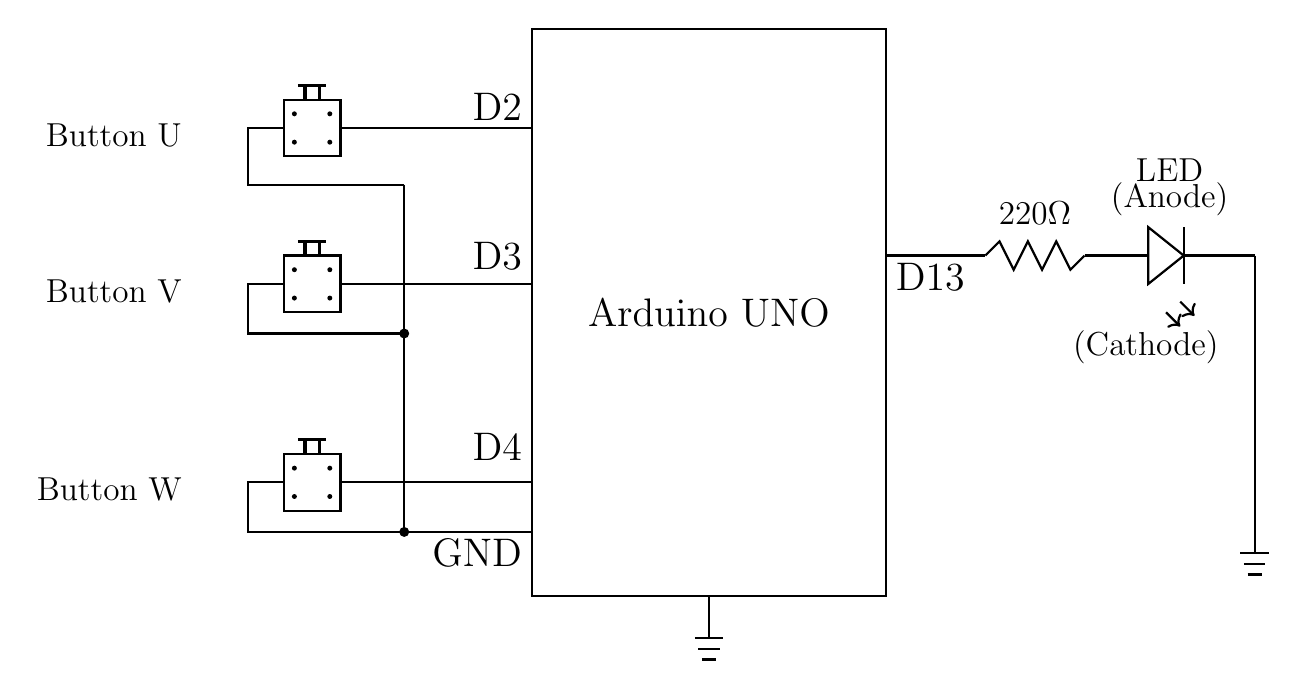
\begin{tikzpicture}[scale=0.90]

% Arduino Block
\draw[thick] (5,0) rectangle (10,8);

\node at (7.5,4) {\Large Arduino UNO};

% Left side labels
\node[left] at (5,6.9) {\Large D2};
\node[left] at (5,4.8) {\Large D3};
\node[left] at (5,2.1) {\Large D4};
\node[left] at (5,0.6) {\Large GND};

% Right side label
\node[right] at (10,4.5) {\Large D13};

%-------------------------------------------------
% Button U
%-------------------------------------------------

\node[left] at (0.2,6.5) {\large Button U};
%\node[left] at (0.5,6.5) {\large (U)};

\draw[thick] (1.5,6.2) rectangle (2.3,7.0);

\fill (1.65,6.4) circle (1pt);
\fill (2.15,6.4) circle (1pt);
\fill (1.65,6.8) circle (1pt);
\fill (2.15,6.8) circle (1pt);

\draw[line width=1.2pt] (1.8,7.0) -- (1.8,7.2);
\draw[line width=1.2pt] (2.0,7.0) -- (2.0,7.2);
\draw[line width=1.2pt] (1.7,7.2) -- (2.1,7.2);

\draw[thick] (2.3,6.6) -- (5,6.6);
\draw[thick] (1.5,6.6) -- (1.0,6.6) -- (1.0,5.8) -- (3.2,5.8);

%-------------------------------------------------
% Button V
%-------------------------------------------------

\node[left] at (0.2,4.3) {\large Button V};
%\node[left] at (0.5,4.3) {\large (V)};

\draw[thick] (1.5,4.0) rectangle (2.3,4.8);

\fill (1.65,4.2) circle (1pt);
\fill (2.15,4.2) circle (1pt);
\fill (1.65,4.6) circle (1pt);
\fill (2.15,4.6) circle (1pt);

\draw[line width=1.2pt] (1.8,4.8) -- (1.8,5.0);
\draw[line width=1.2pt] (2.0,4.8) -- (2.0,5.0);
\draw[line width=1.2pt] (1.7,5.0) -- (2.1,5.0);

\draw[thick] (2.3,4.4) -- (5,4.4);
\draw[thick] (1.5,4.4) -- (1.0,4.4) -- (1.0,3.7) -- (3.2,3.7);

%-------------------------------------------------
% Button W
%-------------------------------------------------

\node[left] at (0.2,1.5) {\large Button W};
%\node[left] at (0.5,1.5) {\large (W)};

\draw[thick] (1.5,1.2) rectangle (2.3,2.0);

\fill (1.65,1.4) circle (1pt);
\fill (2.15,1.4) circle (1pt);
\fill (1.65,1.8) circle (1pt);
\fill (2.15,1.8) circle (1pt);

\draw[line width=1.2pt] (1.8,2.0) -- (1.8,2.2);
\draw[line width=1.2pt] (2.0,2.0) -- (2.0,2.2);
\draw[line width=1.2pt] (1.7,2.2) -- (2.1,2.2);

\draw[thick] (2.3,1.6) -- (5,1.6);
\draw[thick] (1.5,1.6) -- (1.0,1.6) -- (1.0,0.9) -- (3.2,0.9);

%-------------------------------------------------
% Common GND Bus
%-------------------------------------------------

\draw[thick] (3.2,5.8) -- (3.2,0.9);
\fill (3.2,3.7) circle (2pt);
\fill (3.2,0.9) circle (2pt);

\draw[thick] (3.2,0.9) -- (5,0.9);

%-------------------------------------------------
% LED + Resistor
%-------------------------------------------------

\draw[thick] (10,4.8) -- (11.4,4.8);

% Resistor
\draw[thick]
(11.4,4.8)
-- (11.6,5.0)
-- (11.8,4.6)
-- (12.0,5.0)
-- (12.2,4.6)
-- (12.4,5.0)
-- (12.6,4.6)
-- (12.8,4.8);

\node at (12.1,5.4) {\large 220$\Omega$};

\draw[thick] (12.8,4.8) -- (13.7,4.8);

% LED
\draw[thick] (13.7,4.4) -- (13.7,5.2) -- (14.2,4.8) -- cycle;
\draw[thick] (14.2,4.4) -- (14.2,5.2);

\draw[->,thick] (13.95,4.0) -- (14.15,3.8);
\draw[->,thick] (14.15,4.15) -- (14.35,3.95);

\node at (14.0,6.0) {\large LED};
\node at (14.0,5.6) {\large (Anode)};

% GND line
\draw[thick] (14.2,4.8) -- (15.2,4.8);
\draw[thick] (15.2,4.8) -- (15.2,1.2);

\node[right] at (12.5,3.5) {\large (Cathode)};

% Ground Symbol
\draw[thick] (15.2,1.2) -- (15.2,0.6);
\draw[thick] (15.0,0.6) -- (15.4,0.6);
\draw[thick] (15.05,0.45) -- (15.35,0.45);
\draw[thick] (15.1,0.3) -- (15.3,0.3);

% Arduino GND Symbol
\draw[thick] (7.5,0) -- (7.5,-0.6);
\draw[thick] (7.3,-0.6) -- (7.7,-0.6);
\draw[thick] (7.35,-0.75) -- (7.65,-0.75);
\draw[thick] (7.4,-0.9) -- (7.6,-0.9);

\end{tikzpicture}
\caption{Hardware Connection Diagram}
\end{figure}
\subsection{Working Principle}

The Arduino UNO continuously reads the states of the three input switches connected to pins D2, D3, and D4. Since the inputs are configured using \texttt{INPUT\_PULLUP}, pressing a switch produces a logic HIGH after software inversion.

The Arduino evaluates the Boolean expression

\[
I = U(V + \overline{W})
\]

and sends the result to the LED connected to pin D13.

When the expression evaluates to logic HIGH, the LED turns ON. When the expression evaluates to logic LOW, the LED remains OFF.

The values of $U$, $V$, $W$, and the corresponding output $I$ are also displayed on the Serial Monitor, allowing real-time verification of the logic circuit operation.

\section{{Arduino Program}}
\begin{center}
  \small\textcolor{DarkGray}{Full source code on GitHub:\enspace}
  \href{https://github.com/Bheemrajpaidipelli/IITH-Research-May/blob/main/gateproblem.ino}%
       {\textcolor{AccentTeal}{\texttt{https://github.com/Bheemrajpaidipelli/IITH-Research-May/blob/main/gateproblem.ino}}}
\end{center}
\section{Assembly Program}
\begin{center}
  \small\textcolor{DarkGray}{Full source code on GitHub:\enspace}
  \href{https://github.com/Bheemrajpaidipelli/IITH-Research-May/blob/main/gateproblem.asm}%
       {\textcolor{AccentTeal}{\texttt{https://github.com/Bheemrajpaidipelli/IITH-Research-May/blob/main/gateproblem.asm}}}
\end{center}
\section{Results}

\begin{tcolorbox}[resultbox, title={\faFlask\enspace Experimental Findings}]
The Arduino UNO successfully evaluated the simplified Boolean expression for
all possible combinations of the input variables $U$, $V$, and $W$. In each
case, the output LED connected to pin \texttt{D13} produced the expected logic
state, experimentally confirming:

\[
  \boldsymbol{I = U(V + \overline{W})}
\]

Both the C++ (Arduino) implementation and the AVR Assembly implementation
produced identical results, demonstrating consistency across both levels of
abstraction.
\end{tcolorbox}

\section{Optimisation Analysis}

\subsection{Gate Count Comparison}

\begin{table}[H]
\centering
\begin{tabular}{lcc}
\toprule
\textbf{Metric} &
\textbf{Original Expression} &
\textbf{Simplified Expression} \\
\midrule
OR Operations & 3 & 1 \\
NOT Operations & 2 & 1 \\
AND Operations & 2 & 1 \\
Logic Levels & 3 & 2 \\
Implementation & Complex Logic & Reduced Logic \\
\bottomrule
\end{tabular}
\caption{Original Expression vs.\ Simplified Expression}
\end{table}

\subsection{Advantages of Simplification}

\begin{itemize}
    \item \textbf{Reduced logic complexity} --- the original Boolean expression is simplified to a more compact form.

    \item \textbf{Fewer logical operations} --- the number of OR, NOT, and AND operations is reduced.

    \item \textbf{Lower propagation delay} --- fewer logic levels result in faster output generation.

    \item \textbf{Simpler implementation} --- the simplified expression is easier to implement in both hardware and software.

    \item \textbf{Improved readability} --- the simplified equation is easier to understand, analyse, and debug.

    \item \textbf{Efficient resource utilisation} --- fewer logic operations require less computational effort during execution.
\end{itemize}

\section{Conclusion}

The given logic circuit was successfully analysed and the corresponding Boolean
expression was derived from the circuit diagram. Using Boolean algebra, the
expression was simplified to

\[
I = U(V + \overline{W})
\]

The simplified expression was implemented using an Arduino UNO and verified
experimentally using push-button inputs and an LED output. The observed output
matched the expected truth table values for all possible input combinations,
confirming the correctness of both the circuit analysis and the simplification
process.

The AVR Assembly implementation also produced identical results, demonstrating
consistency between high-level and low-level implementations. This project
highlights the importance of Boolean simplification in reducing logic complexity,
improving implementation efficiency, and facilitating the design and verification
of digital electronic systems.

\vfill
\begin{center}
  \textcolor{MidGray}{\small --- End of Report ---}
\end{center}

\end{document}
